\documentclass{article} 
\usepackage{amsmath}
\usepackage{amssymb}
\usepackage{enumerate}
\usepackage[unicode]{hyperref}
\hypersetup{
	colorlinks,
	citecolor=black,
	filecolor=black,
	linkcolor=black,
	urlcolor=blue
}
\usepackage{chngcntr}
\counterwithin{figure}{section}
\usepackage[top=2cm, bottom=2cm, left = 3cm, right = 2cm]{geometry}
\usepackage{graphicx}
\usepackage{multirow}
\usepackage{textcase}
\usepackage[utf8]{vietnam}
\usepackage{booktabs}
\usepackage{adjustbox}
\usepackage{listings}
\usepackage{color}
\usepackage{ dsfont }
\usepackage{makeidx}
\usepackage[table,xcdraw]{xcolor}
\makeindex
\definecolor{dkgreen}{rgb}{0,0.6,0}
\definecolor{gray}{rgb}{0.5,0.5,0.5}
\definecolor{mauve}{rgb}{0.58,0,0.82}

\lstset{frame=tb,
  language=Java,
  aboveskip=3mm,
  belowskip=3mm,
  showstringspaces=false,
  columns=flexible,
  basicstyle={\small\ttfamily},
  numbers=none,
  numberstyle=\tiny\color{gray},
  keywordstyle=\color{blue},
  commentstyle=\color{dkgreen},
  stringstyle=\color{mauve},
  breaklines=true,
  breakatwhitespace=true,
  tabsize=3
}
\lstset
{language=Python}
\title{Tìm hiểu về thuật toán K-Means} 
\author{Nguyễn Văn Huy \& Lê Duy An} 
\begin{document}
	\maketitle{} 
	\newpage
	\tableofcontents
	\newpage
	\section{Giới thiệu}
	Phân cụm là kỹ thuật rất quan trọng trong việc khai thác dữ liệu. Phân cụm là các quy trình tìm cách nhóm các đối tượng đã cho vào các cụm (clusters), sao cho các đối tượng trong cùng 1 cụm thoả mãn các tính chất tương tự nhau và các đối tượng khác cụm thì không tương tự nhau.\par
	\smallskip
	Kỹ thuật phân cụm có thể được áp dụng trong đa dạng các lĩnh vực khác nhau như:
	\begin{itemize}
		\item Marketing: Xác định các nhóm khách hàng dựa trên sở thích, thói quen mua sắm,...
		\item Sinh học: Phận nhóm động vật và thực vật dựa vào các thuộc tính của chúng,...
		\item Quản lý thư viện: Theo dõi độc giả, sách, dự đoán nhu cầu của độc giả,...
		\item Giao thông: tìm nhóm đường có tốc độ giống nhau,...
		\item ...
	\end{itemize}
	Phương pháp k-means là một trong số những thuật toán phân cụm (clustering). Với đầu vào tập dữ liệu cần phân cụm và số cụm (cluster), đầu ra chúng ta sẽ được kết quả dữ liệu đã được phân về các cluster.\par
	\smallskip
	Trong thuật toán K-means clustering, chúng ta không biết nhãn (label) của từng điểm dữ liệu. Mục đích là làm thể nào để phân dữ liệu thành các cụm (cluster) khác nhau sao cho dữ liệu trong cùng một cụm có tính chất giống nhau.\par
	\smallskip
	\begin{figure}[h]
		\centering
		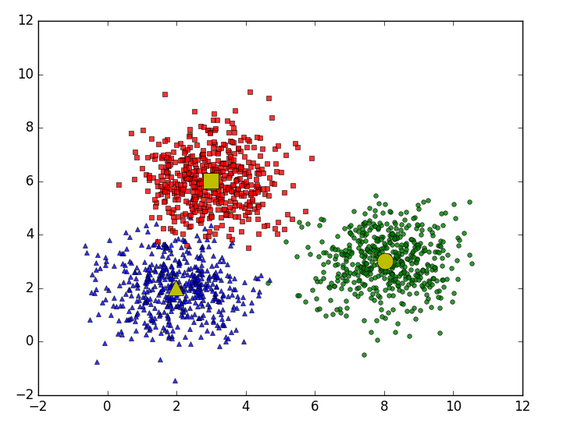
\includegraphics[width=0.7\linewidth]{img/cluster_ex}
		\caption{Ví dụ về bài toán phân cụm dữ liệu}
	\end{figure}\par
	Xem xét ví dụ về các phân cụm dữ liệu như hình trên, ta quan sát được mỗi cụm có một điểm màu vàng gọi là điểm trung tâm (centroid), các điểm dữ liệu nằm gần điểm trung tâm nào nhất thì thuộc cùng một nhóm với điểm trung tâm đó. Như vậy, từ một bộ dữ liệu ban đầu, ta đã phân thành 3 cụm dữ liệu, mỗi cụm bao gồm các điểm dữ liệu có tính chất tương tự nhau.
	\newpage
	\section{Phân tích toán học} % (fold)
	\label{sec:phân_tích_toán_học}
	Với dữ liệu đầu vào của thuật toán là tập hợp các điểm dữ liệu $\mathbf{X} = [\mathbf{x}_1,\mathbf{x}_2,\mathbf{x}_3,...,\mathbf{x}_N]$ $\in \mathds{R}^{d\times N}$ với $\mathbf{x}_i$ (có $d$ phần tử) là một vector mang giá trị của mỗi điểm, $N$ là số lượng các vector và số lượng $K$ các nhóm cần phân loại từ các điểm dữ liệu đó với $K < N$ (vì số lượng nhóm cần phân loại không được lớn hơn số lượng các phần tử). Điều mà chúng ta cần phải làm là làm thế nào để xác định các điểm thuộc về nhóm nào một cách gắn kết nhất, ở đây để cho dễ gọi và tính toán thì chúng ta cho rằng $K$ nhóm cần phần loại được gọi là nhóm $1,2,3,..K$. Trong phần này chúng ta chỉ đề cập đến bài toán chỉ có một điểm dữ liệu thuộc vào một nhóm duy nhất.
	\\
	Ban đầu chúng ta phải có được các điểm gốc ban đầu của các nhóm có thể chọn $k$ điểm bất kì hoặc có thể lấy các điểm dữ liệu có sẵn trong tập dữ liệu ban đầu. Gọi các điểm gốc ban đầu là $\mathbf{m} = [\mathbf{m}_1,\mathbf{m}_2,\mathbf{m}_3,...,\mathbf{m}_K]$ với mỗi điểm $\mathbf{m}_k$ cũng có có $d$ các giá trị tương tự như các điểm dữ liệu $\mathbf{x}_i$. Dựa vào tập các điểm gốc $\mathbf{m}_k$ chúng ta phải xác định xem điểm $\mathbf{x}_i$ thuộc vào nhóm nào và gán nhãn cho các điểm đó bằng vector $\mathbf{y}$ có dạng:
	% \begin{center}
	$$\mathbf{y}_{ij} \in \{0,1\},\ \forall i,j;\ \  \sum_{j = 1}^{K} = 1,\  \forall i$$
	% \end{center}
	Trong đó $\mathbf{y}_{ij} = 0$ và $\mathbf{y}_{ik} = 1$, nghĩa là vector $\mathbf{y}$ có $K$ giá trị và vị trí ở vị trí $k$ có giá trị bằng 1 thì đồng nghĩa là vector $\mathbf{x}_i$ được gán vào nhóm $k$. Tập hợp các nhãn là $\mathbf{Y} = [\mathbf{y}_1,\mathbf{y}_2,\mathbf{y}_3,...,\mathbf{y}_N]$ $\in \mathds{R}^{K\times N}$.
	% \\
	% $$
	\\ 
	Một ví dụ để hình dung rõ hơn về các tập dữ liệu. Ví dụ đề cập đến việc phân nhóm các điểm của tập $\mathbf{X} = [\mathbf{x}_1,\mathbf{x}_2,\mathbf{x}_3,...,\mathbf{x}_N]$ được biễu diễn trong Bảng \ref{tab:tbexample} nằm trong  không gian $2\mathds{D}$ gồm có số lượng các điểm là $N = 20$ được biểu diễn trong Hình \ref{fig:example1} bằng các điểm màu xanh, vì trong không gian $2\mathds{D}$ nên $d = 2$ tương ứng là tọa độ $x$ và $y$. Điều kiện của bài toán là các điểm đó thành ba cụm với ba điểm ban đầu là $\mathbf{m} = [(1;17),(3;4),(5;15)]$ có $K = 3$ được biểu thị bằng các điểm màu đỏ trên Hình \ref{fig:example1}.
	
	\begin{figure}[h]
		\centering
		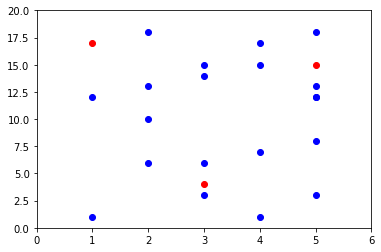
\includegraphics[width=0.5\linewidth]{img/img_example}
		\caption{Hình các các dữ liệu đầu vào.}
		\label{fig:example1}
	\end{figure}
	
	\begin{table}[h]
		\centering
		\begin{tabular}{|c|c|c|}
			\hline
			$\mathbf{X}$                       & $x$                      & $y$                       \\ \hline
			$\mathbf{x}_1$                       & 1                      & 4                       \\ \hline
			$\mathbf{x}_2$                       & 5                      & 12                      \\ \hline
			$\mathbf{x}_3$                       & 2                      & 18                      \\ \hline
			...                       & ...                      & ...                      \\ \hline
			\multicolumn{1}{|l|}{$\mathbf{x}_N$}   & \multicolumn{1}{l|}{5} & \multicolumn{1}{l|}{13} \\ \hline
			% ...                     &                        &                         \\ \hline
		\end{tabular}
		\caption{Bảng biểu diễn một vài giá trị của các điểm trong tập $\mathbf{X}$}
		\label{tab:tbexample}
	\end{table}\par
	\begin{table}[h]
		\centering
		\begin{tabular}{|c|c|c|c|}
			\hline
			$\mathbf{Y}$                           & 1                      & 2                       & 3                       \\ \hline
			$\mathbf{y}_1$                         & 0                      & 0                       & 1                       \\ \hline
			$\mathbf{y}_2$                         & 1                      & 0                       & 0                       \\ \hline
			$\mathbf{y}_3$                         & 0                      & 1                       & 0                       \\ \hline
			...                                    & ...                    & ...                     & ...                     \\ \hline
			\multicolumn{1}{|l|}{$\mathbf{y}_N$}   & \multicolumn{1}{l|}{0} & \multicolumn{1}{l|}{0}  & \multicolumn{1}{l|}{1}  \\ \hline
			% ...                     &                        &                         \\ \hline
		\end{tabular}
		\caption{Bảng biểu diễn mội vài nhãn $\mathbf{y}_i$ trong tập $\mathbf{Y}$}
		\label{tab:tbexample}
	\end{table}\par
	\newpage
	\subsection{Hàm mất mát và bài toán tối ưu} % (fold)
	Nếu gọi $m_k \in \mathbb{R}^d$ là centroid của mỗi cluster và thay thế tất cả các điểm được phân vào cluster này bởi $m_k$, một điểm dữ liệu $x_i$ được phân vào cluster k sẽ bị sai số là $x_i - m_k$. CHúng ta mong muốn vector sai số này gần với vector không, tức $x_i$ gần với $m_k$. Một đại lượng đơn giản giúp đo khoảng cách giữa hai điểm là khoảng cách Euclid $||x_i - m_k||^2_2$. Hơn nữa, vì $x_i$ được phân vào cluster k nên $y_{ik} = 1, y_{ij} = 0, \forall j \neq k}$. Khi đó, biểu thức khoảng cách Euclid có thể được viết lại thành\par
	\begin{center}
		$||x_i - m_k||^2_2 = y_{ik}||x_i - m_k||^2_2 = \sum\limits^K_{j = 1}{y_{ij}||x_i - m_k||^2_2}$
	\end{center}
	\subsection{Thuật toán tối ưu hàm mất mát}
	\newpage
	\section{Ưu và nhược điểm} % (fold)
	\subsection{Ưu điểm}
	\begin{itemize}
		\item Thuật toán đơn giản, hiệu quả với độ phức tạo là $O(tKn)$, t, k << n, với:
		\item[--]t: số lần lặp
		\item[--]K: số cluster
		\item[--]n: số mẫu
		\item Sử dụng được với bộ số liệu lớn
	\end{itemize}
\subsection{Nhược điểm}
\begin{itemize}
	\item Cần phải xác định trước số lượng cluster. Trong thực tế, cần phải sử dụng thêm một số biện pháp giúp xác định giá trị K, chẳng hạn như phương pháp Elbow.
	\item Thuật toán KMeans không đảm bảo tìm được nghiệm tối ưu toàn cục nên nghiệm cuối cùng phụ thuộc rất nhiều vào các centroid ban đầu. Hình 3.1 thể hiện các kết quả khác nhau khi các centroid khởi tạo khác nhau. Ngoài ra, việc chọn các centroid cũng ảnh hưởng đến hiệu suất làm việc của thuật toán. Với cùng một kết quả tối ưu như nhau, số lần chạy ở hình 2 lớn gần gấp đôi so với hình 1.\\
	\begin{figure}[h]
		\centering
		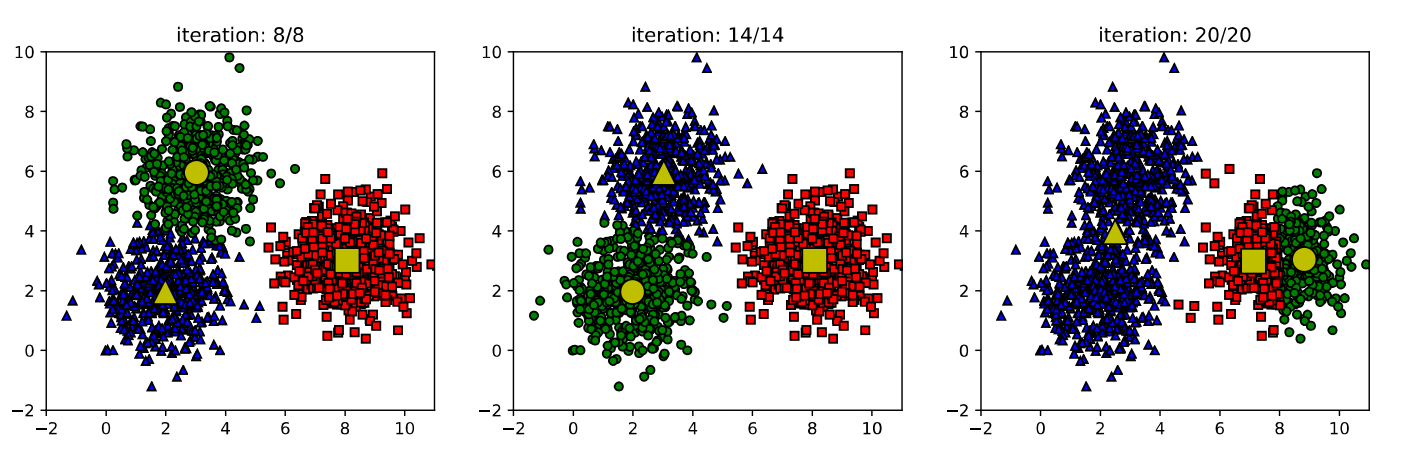
\includegraphics[width=0.7\linewidth]{img/disad_1}
		\label{dis1}
		\caption{Các nghiệm khác nhau do khởi tạo ban đầu khác nhau}
	\end{figure}
	\item Các cluster cần phải có số lượng điểm gần bằng nhau. Ở hình 3.2 minh hoạ kết quả thuật toán KMeans với bộ dữ liệu có các cluster có số điểm chênh lệch. Trong trường hợp này, nhiều điểm đáng lẽ thuộc vào cụm xanh lam đã bị nhầm vào cụm xanh lục.\par
	\begin{figure}[h]
		\centering
		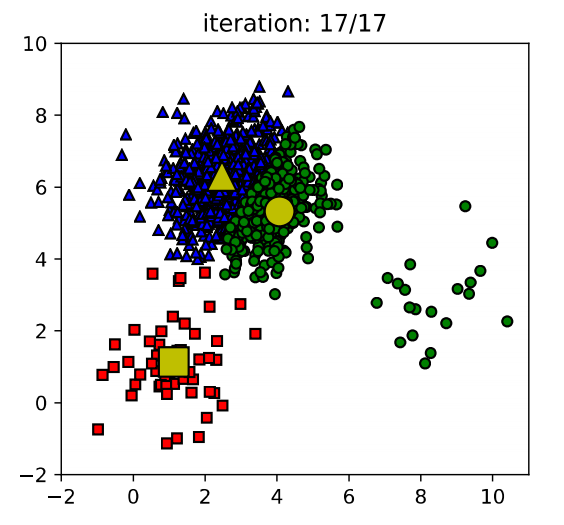
\includegraphics[width=0.3\linewidth]{img/disad_2}
		\caption{Các nghiệm trong cluster này bị nhầm vào cluster khác}
	\end{figure}\par
	\item Các cluster cần có dạng hình tròn (cầu), nếu không thì KMeans sẽ hoạt động không hiệu quả. Lý do chính là vì Kmeans quyết định cluster của một điểm dữ liệu thông qua khoảng cách của nó đến centroid.	
	\begin{figure}[h]
		\centering
		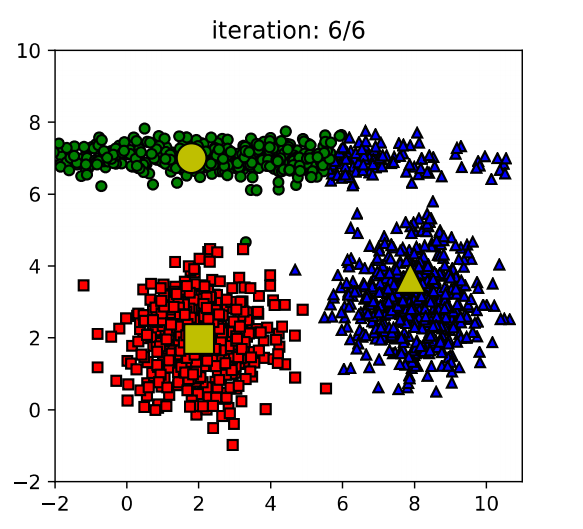
\includegraphics[width=0.3\linewidth]{img/disad_3}
		\caption{Các nghiệm trong cluster này bị nhầm vào cluster khác}
	\end{figure}
	\item Centroid có thể bị xê dịch bởi các ngoại lệ, hoặc các ngoại lệ có thể có cụm riêng thay vì bị bỏ qua.
	\item Cho kết quả sai khi một cluster này bị bao bọc bằng một cluster khác. Hình 3.3 là một minh hoạ điển hình cho việc KMeans không thể phân cụm dữ liệu. Một cách tự nhiên, chúng ta chia hình mặt thành 4 cụm: mắt trái, mắt phải, miệng, hình bao quanh mặt. Nhưng vì các bộ phận mắt, miệng nằm bên trong mặt nên KMeans phân cụm không chính xác.
	\begin{figure}[h]
		\centering
		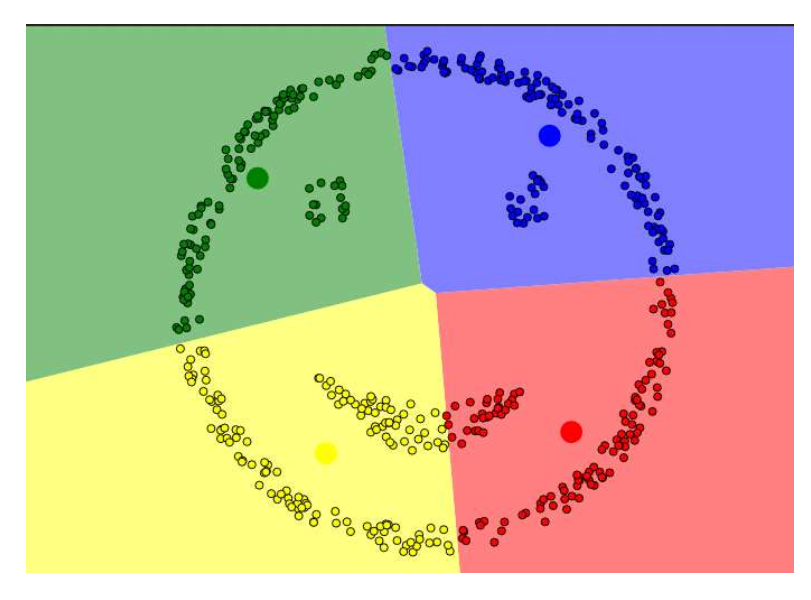
\includegraphics[width=0.5\linewidth]{img/disad_4}
		\caption{KMeans phân cụm hình mặt không chính xác}
	\end{figure}	
	\end{itemize}
	\section{Cách tìm K cụm tối ưu nhất}
	Xác định số lượng cụm tối ưu trong một tập dữ liệu là vấn đề cơ bản trong phân cụm Kmeans, yêu cầu người dùng chỉ định số lượng cụm k được tạo. Ý tưởng đằng sau Kmeans bao gồm xác định các cụm k sao cho tổng biến thể trong cụm là tối thiểu. Đây được xem là một nhược điểm của thuật toán này. Phần dưới đây trình bày một vài phương pháp giúp xác định số cụm k hợp lý nhất.\par
	\subsection{Thuật toán Elbow}
	Tư tưởng chính của phương pháp phân cụm phân hoạch (như KMeans) là định nghĩa 1 cụm sao cho tổng bình phương khoảng cách của tất cả các điểm đến đến trung tâm cụm là nhỏ nhất, tham số này là WSS (Within-cluster Sum of Square). Elbow method chọn số cụm k sao cho khi thêm vào  một cụm khác thì không làm cho WSS thay đổi nhiều.\par
	\newpage
	Quy trình triển khai thuật toán Elbow:
	\begin{itemize}
		\item Thực hiện phân cụm với số cụm thay đổi
		\item Với mỗi giá trị k, tính giá trị WSS
		\item Vẽ đường cong Elbow theo các giá trị k
		\item Dựa vào đường cong Elbow chọn số k thích hợp, là vị trí ở khúc cua 
	\end{itemize}
	Xét ví dụ mẫu dữ liệu sau:
	\begin{figure}[h]
		\centering
		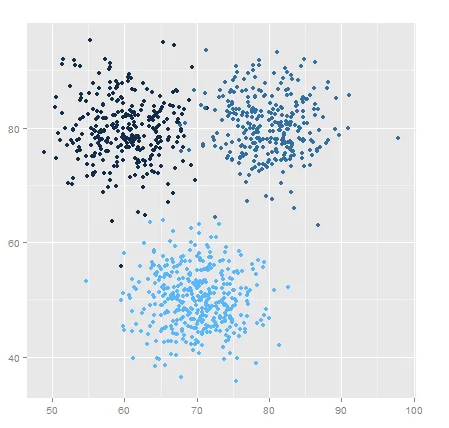
\includegraphics[width=0.5\linewidth]{img/data_set_1}
		\caption{Mẫu dữ liệu}
	\end{figure}\par
	Tính toán giá trị WSS tương ứng với K từ 1 đến 20, ta thu được biểu đồ sau:
	\begin{figure}[h]
		\centering
		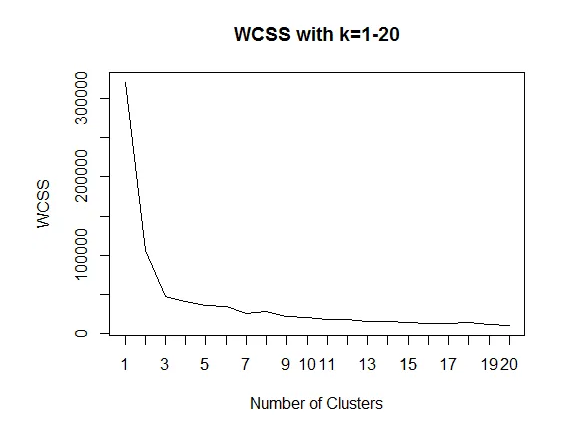
\includegraphics[width=0.6\linewidth]{img/data_set_2}
		\caption{WSS tương ứng với k từ 1 đến 20}
	\end{figure}\par
	Ta chọn k = 3 làm số cụm cho mẫu dữ liệu trên.
	\newpage
	\subsection{Thuật toán Average Silhouette}
	Average silhouette dùng để đo chất lượng của một cụm. Giá trị Silhouette s(i) cho mỗi điểm dữ liệu i được xác định như sau:\\
	\begin{center}
		\large
		$s(i) = \frac{b(i) - a(i)}{max\{a(i), b(i)\}} (|C_i| > 1)$
	\end{center}\par
	Trong đó:
	\begin{itemize}
		\item a(i) khoảng cách trung bình từ điểm i đến các điểm khác trong cụm. $a(i) = \frac{1}{|C_i| - 1}\sum\limits_{j \in C_i, i \neq j}{d(i, j)}$
		\item b(i) là khoảng cách trung bình giữa các cụm. $b(i) = \underset{i \neq j}{min} \frac{1}{|C_j|}\sum\limits_{j \in C_j}{d(i, j)}$
	\end{itemize}\par
	Với s(i) = 0 với những cụm có chỉ có 1 phần tử.\par
	\smallskip
	Quy trình triển khai thuật toán average silhouette:
	\begin{itemize}
		\item Thực hiện phân cụm với số cụm thay đổi
		\item Với mỗi giá trị k, tính giá trị average silhouette
		\item Vẽ đường cong average silhouette theo các giá trị k
		\item Vị trí có average silhouette lớn nhất là số cụm cần tìm
	\end{itemize}
	Xét ví dụ về mẫu dữ liệu sau:
	\begin{figure}[h]
		\centering
		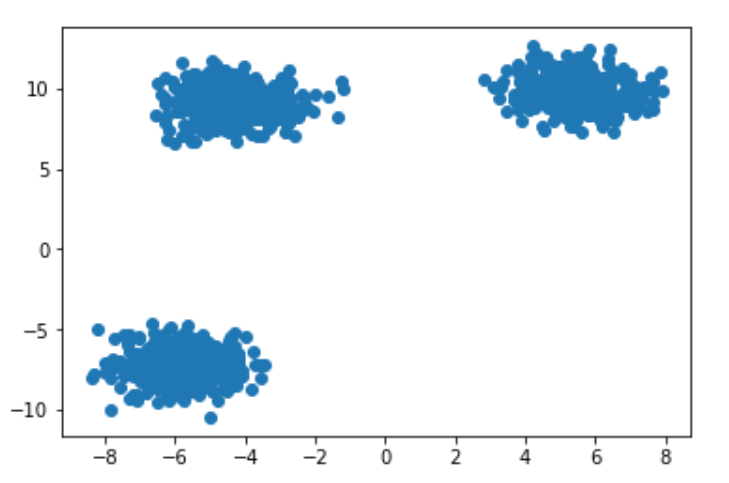
\includegraphics[width=0.5\linewidth]{img/data_set_3}
		\caption{Mẫu dữ liệu}
	\end{figure}\par
	Vẽ đường cong average silhouette:\par
	\begin{figure}[h]
		\centering
		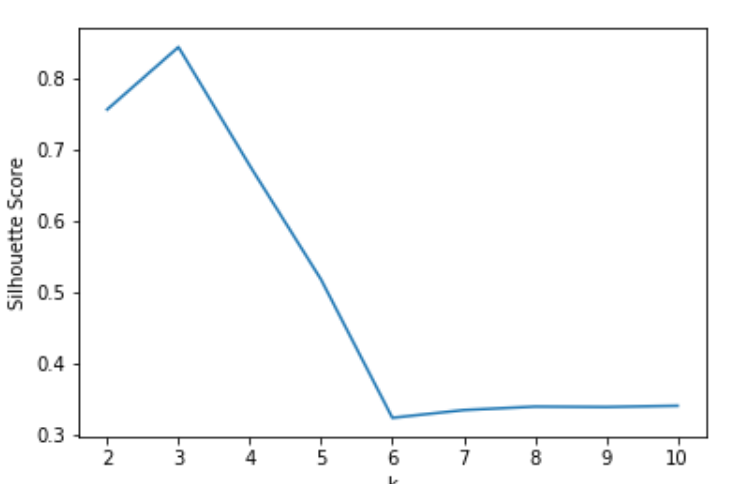
\includegraphics[width=0.5\linewidth]{img/data_set_4}
	\end{figure}\par
	Ta chọn k = 3 làm số cụm cho mẫu dữ liệu trên.
\end{document}